% Search for all the places that say "PUT SOMETHING HERE".

\documentclass[11pt]{article}
\usepackage{amsmath,textcomp,amssymb,graphicx,enumerate,hyperref,enumitem,mathtools,tikz-qtree,listings,chemformula,bm,graphicx,grffile,gensymb}
\graphicspath{{/Users/jonathansun5/Documents/Fall 2017/MCB 166/Homeworks/HW 2/Screen Shot 2017-10-02 at 2.51.29 AM.png}}

\makeatletter
\newcommand{\leqnos}{\tagsleft@true\let\veqno\@@leqno}
\newcommand{\reqnos}{\tagsleft@false\let\veqno\@@eqno}
\reqnos
\makeatother

\def\Name{Jonathan Sun}  % Your name
\def\SID{25020651}  % Your student ID number
\def\Homework{2} % Number of Homework
\def\Session{Fall 2017}


\title{MCB166 --- \Session --- Problem Set \Homework}
\author{\Name, SID \SID}
\markboth{MCB166 --- \Session --- Problem Set \Homework --- \Name}{MCB166 --- \Session --- Problem Set \Homework --- \Name}
\pagestyle{myheadings}
\date{}

\def\endproofmark{$\Box$}
\newenvironment{proof}{\par{\bf Proof:}}{\endproofmark\smallskip}

\usepackage[margin=1in]{geometry}



\begin{document}
\maketitle

\newpage
\begin{enumerate}[label=\arabic*.]
\item
\underline{Threshold-switch model of excitation}
\vspace*{1\baselineskip}
\\










\newpage
\item
\underline{Strength-Duration Relation} (Lapique's Law)
\vspace*{1\baselineskip}
\\
For constant-current stimuli, the amplitude and duration of the stimulating current step are related by Lapique's Law,
\begin{align*}
I\text{*} = I_{Rh} / (1 - \text{exp}(-t\text{*} / T))
\end{align*}
$I_{Rh}$, called the rheobase is the minimum current which can cause excitation. T is the membrane the characteristic membrane time constant.
\vspace*{1\baselineskip}
\\
Using the current-clamp response to the different current steps (ie. the results of prob. 1), derive Lapique's law (ie. calculate the time it takes for the voltage to reach V\text{*} as a function of stimulus amplitude, I\text{*} and the time to reach threshold for that particular stimulus, t\text{*}).
\vspace*{1\baselineskip}
\\
To solve this problem, we start with:
\begin{align*}
V(t_\theta) = V_\theta = E_r + \frac{I} {G_r} \left(1 - e ^ {\frac{-t_\theta} {\tau}}\right)
\end{align*}
Which I will rewrite as:
\begin{align*}
V\text{*} = E_r + \frac{I\text{*}} {G_r} \left(1 - e ^ {\frac{-t\text{*}} {T}}\right)
\end{align*}
\begin{align*}
V\text{*} - E_r = \frac{I\text{*}} {G_r} \left(1 - e ^ {\frac{-t\text{*}} {T}}\right)
\end{align*}
\begin{align*}
G_r \left(V\text{*} - E_r\right) = I\text{*} \left(1 - e ^ {\frac{-t\text{*}} {T}}\right)
\end{align*}
From problem 1, we were given that:
\begin{align*}
I_{Rh} = G_r \left(V\text{*} - E_r\right)
\end{align*}
Therefore, we can rewrite the equation as:
\begin{align*}
I_{Rh} = I\text{*} \left(1 - e ^ {\frac{-t\text{*}} {T}}\right)
\end{align*}
\begin{align*}
I\text{*} = \frac{I_{Rh}} {1 - e ^ {\frac{-t\text{*}} {T}}}
\end{align*}
Therefore, we have derived Lapique's law using the current-clamp response to different current steps.



\newpage
\item
\underline{Equivalent Circuit with Electrogenic Pump}
\begin{center}
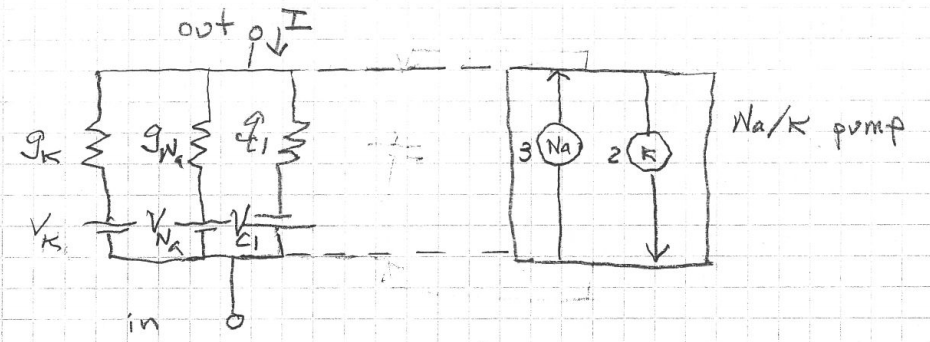
\includegraphics[width=1\textwidth]{/Users/jonathansun5/Documents/Fall 2017/MCB 166/Homeworks/HW 2/Screen Shot 2017-10-02 at 2.51.29 AM.png}
\end{center}
The figure shows the equivalent circuit for an axon at rest in parallel with an equivalent constant-current source representing the \ch{Na+}/\ch{K+}-ATPase pump.
\begin{enumerate}[label=(\alph*)]
\item
Write an expression for the reversal potential (in the absence of the pump) in terms of $V_{\ch{K}}$, $V_{\ch{Na}}$, $V_{\ch{Cl}}$ and the \underline{relative} conductances
\begin{align*}
\alpha = g_{\ch{Na}} / g_{\ch{K}} \text{ and } \beta = g_{\ch{Cl}} / g_{\ch{K}}.
\end{align*}
Is this situation, $I_{\ch{L}} = I_{\ch{K}} + I_{\ch{Na}} + I_{\ch{Cl}} = 0$, an equilibrium? If not, why not?
\vspace*{1\baselineskip}
\\
To solve this problem, we start with:
\begin{align*}
I_{total} = G_{\ch{K}} \left(V_r - E_{\ch{K}}\right) + G_{\ch{Na}} \left(V_r - E_{\ch{Na}}\right) + G_{\ch{Cl}} \left(V_r - E_{\ch{Cl}}\right) = 0
\end{align*}
\begin{align*}
G_{\ch{K}} V_r - G_{\ch{K}} E_{\ch{K}} + G_{\ch{Na}} V_r - G_{\ch{Na}} E_{\ch{Na}} + G_{\ch{Cl}} V_r - G_{\ch{Cl}} E_{\ch{Cl}} = 0
\end{align*}
\begin{align*}
G_{\ch{K}} V_r + G_{\ch{Na}} V_r + G_{\ch{Cl}} V_r = G_{\ch{K}} E_{\ch{K}} + G_{\ch{Na}} E_{\ch{Na}} + G_{\ch{Cl}} E_{\ch{Cl}}
\end{align*}
Dividing both sides by $G_{\ch{K}}$ gives us:
\begin{align*}
\frac{G_{\ch{K}} V_r + G_{\ch{Na}} V_r + G_{\ch{Cl}} V_r} {G_{\ch{K}}} = \frac {G_{\ch{K}} E_{\ch{K}} + G_{\ch{Na}} E_{\ch{Na}} + G_{\ch{Cl}} E_{\ch{Cl}}} {G_{\ch{K}}}
\end{align*}
\begin{align*}
V_r + \frac{G_{\ch{Na}}} {G_{\ch{K}}} V_r + \frac{G_{\ch{Cl}}} {G_{\ch{K}}} V_r = E_{\ch{K}} + \frac{G_{\ch{Na}}} {G_{\ch{K}}} E_{\ch{Na}} + \frac{G_{\ch{Cl}}} {G_{\ch{K}}} E_{\ch{Cl}}
\end{align*}
Substituting in $\alpha = \frac{g_{\ch{Na}}} {g_{\ch{K}}}$ and $\beta = \frac {g_{\ch{Cl}}} {g_{\ch{K}}}$ gives us:
\begin{align*}
V_r + \alpha V_r + \beta V_r = E_{\ch{K}} + \alpha E_{\ch{Na}} + \beta E_{\ch{Cl}}
\end{align*}
\begin{align*}
V_r = \frac{E_{\ch{K}} + \alpha E_{\ch{Na}} + \beta E_{\ch{Cl}}} {1 + \alpha + \beta}
\end{align*}
If 










\newpage
\item
Now introduce the pump
\begin{align*}
I_{pump} = I_{\ch{Na}-pump} + I_{\ch{K}-pump},
\end{align*}
\begin{align*}
I_{\ch{Na}-pump} =  -\frac{3} {2} I_{\ch{K}-pump}.
\end{align*}
Write the expression for the new resting potential in terms of the batteries and (new) \underline{relative} permeabilities. Use the equilibrium conditions:
\begin{align*}
I_{\ch{Na}} = I_{\ch{Na}-leak} + I_{\ch{Na}-pump}
\end{align*}
\begin{align*}
I_{\ch{K}} = I_{\ch{K}-leak} + I_{\ch{K}-pump},
\end{align*}
\begin{align*}
I_{\ch{Cl}} = 0
\end{align*}
To solve this problem, we start with:
\begin{align*}
I_{pump} = I_{\ch{Na}-pump} + I_{\ch{K}-pump}
\end{align*}
\begin{align*}
I_{pump} = I_{\ch{Na}-leak} + I_{\ch{Na}-pump} + I_{\ch{K}-leak} + I_{\ch{K}-pump} = 0
\end{align*}
\begin{align*}
I_{\ch{Na}-leak} + \left(-\frac{3} {2} I_{\ch{K}-pump}\right) + I_{\ch{K}-leak} + I_{\ch{K}-pump} = 0
\end{align*}
\begin{align*}
I_{\ch{Na}-leak} - \frac{1} {2} I_{\ch{K}-pump} + I_{\ch{K}-leak} = 0
\end{align*}
\begin{align*}
I_{\ch{Na}-leak} + \frac{1} {2} I_{\ch{K}-leak} + I_{\ch{K}-leak} = 0
\end{align*}
\begin{align*}
I_{\ch{Na}-leak} + \frac{3} {2} I_{\ch{K}-leak} = 0
\end{align*}
This equation can be rewritten as:
\begin{align*}
G_{\ch{Na}} \left(V_r - E_{\ch{Na}}\right) + \frac{3} {2} G_{\ch{K}} \left(V_r - E_{\ch{K}}\right) = 0
\end{align*}
\begin{align*}
G_{\ch{Na}} V_r - G_{\ch{Na}} E_{\ch{Na}} + \frac{3} {2} G_{\ch{K}} V_r - \frac{3} {2} G_{\ch{K}} E_{\ch{K}} = 0
\end{align*}
\begin{align*}
G_{\ch{Na}} V_r + \frac{3} {2} G_{\ch{K}} V_r = G_{\ch{Na}} E_{\ch{Na}} + \frac{3} {2} G_{\ch{K}} E_{\ch{K}}
\end{align*}
\begin{align*}
V_r = \frac{G_{\ch{Na}} E_{\ch{Na}} + \frac{3} {2} G_{\ch{K}} E_{\ch{K}}} {G_{\ch{Na}} + \frac{3} {2} G_{\ch{K}}}
\end{align*}









\newpage
\item
Show that the formula you derived is still valid when you ignore the chloride terms (as I did in the worked example\text{*}). Explain this by working out the relation between the equilibrium concentrations of \ch{Cl-} and the membrane potential.
\vspace*{1\baselineskip}
\\
To solve this problem, we start with:
\begin{align*}
I_{\ch{Cl}} = 0
\end{align*}
This equation can be rewritten as:
\begin{align*}
G_{\ch{Cl}} \left(V_r - E_{\ch{Cl}}\right) = 0
\end{align*}
Dividing both sides by $G_{\ch{Cl}}$ gives us:
\begin{align*}
\frac{G_{\ch{Cl}} \left(V_r - E_{\ch{Cl}}\right)} {G_{\ch{Cl}}} = \frac{0} {G_{\ch{Cl}}}
\end{align*}
\begin{align*}
V_r - E_{\ch{Cl}} = 0
\end{align*}
\begin{align*}
V_r = E_{\ch{Cl}}
\end{align*}






\end{enumerate}




% \vspace*{1\baselineskip}
% \\









\end{enumerate}
\end{document}
